%!TEX root = ../bachelor.tex
\chapter{Einleitung}
\todo{einleitung schreiben}
\begin{itemize}
	\item Ausgangssitatuion
	\item Problemstellung
	\item Zielstellung
	\item Methodik
	\item nur eine Kamera statt 5
	\item zur Beobachtung von Drosophila melanogaster - Larven
	\item stressfreie Umgebung als auf dem FIM-Tisch
	\item kein Stitching mehr notwendig, keine synchronsisation
	\item besseres Verhältnis zwischen Gehege und Kameras
	\item keine Ghosts
	\item Entzerrung bleibt
	\item Larven oben wesentlich größer als unten (perspektivische Verzerrung) $\rightarrow$ kein relativer Vergleich der Größe möglich
	\item Verfolgen von Larven, ändern die Größe $\rightarrow$ auch schlecht
	\item Entzerrungsverfahren, dass die 3D - Kegeloberfläche auf die 2D-Mantelfläche abbildet, sodass ein Vergleich möglich ist $\rightarrow$ Thema der Arbeit
	\item zwei verschiedene Verfahren werden vorgestellt?
\end{itemize}

Um die Larven möglichst stressfrei untersuchen zu können werden die Larven in ihrem Aufzuchtröhrchen beobachtet. 

Der bisherige Untersuchungsaufbau ist in Abbildung \ref{fig:oldSetup} abgebildet. Die Larven befinden sich hierbei in einem Zylinder, der von insgesamt fünf Kameras beobachtet wird, die jeweils an einen Raspberry Pi angeschlossen sind. Die Kameras nehmen nun simultan ein Bild auf, wobei hier eine Synchronisation notwendig ist. Auf Grund der Krümmung des Zylinders, müssen diese nun entsprechend entzerrt werden. Anschließend werden die fünf entzerrten Bilder zu einem Gesamtbild zusammengefügt. 
Um ein besseren Verhältnis zwischen der Anzahl der Kameras und Gehege zu erreichen, wäre eine Reduktion Kameraanzahl wünschenswert. 
Statt eines Zylinders benutzen wir nun einen Kegel, wie in Abbildung \ref{fig:newSetup} zu sehen, und beobachten den Aufbau mit einer einzigen Kamera. Wie auch bei dem bisherigen Aufbau muss hier eine Entzerrung stattfinden. Die Larven, die sich am oberen Rand des Kegels bewegen scheinen sonst größer, als jene, die sich im unteren Bereich aufhalten. Eine Synchronisation ist jedoch nicht mehr notwendig. 

oder wir stellen zwei vor
Ziel dieser Arbeit ist die Entwicklung eines Verfahrens zur Entzerrung von Kegeloberflächen. 

\begin{figure}[!htb]
	\centering
	\begin{subfigure}{.5\textwidth}
		\centering
		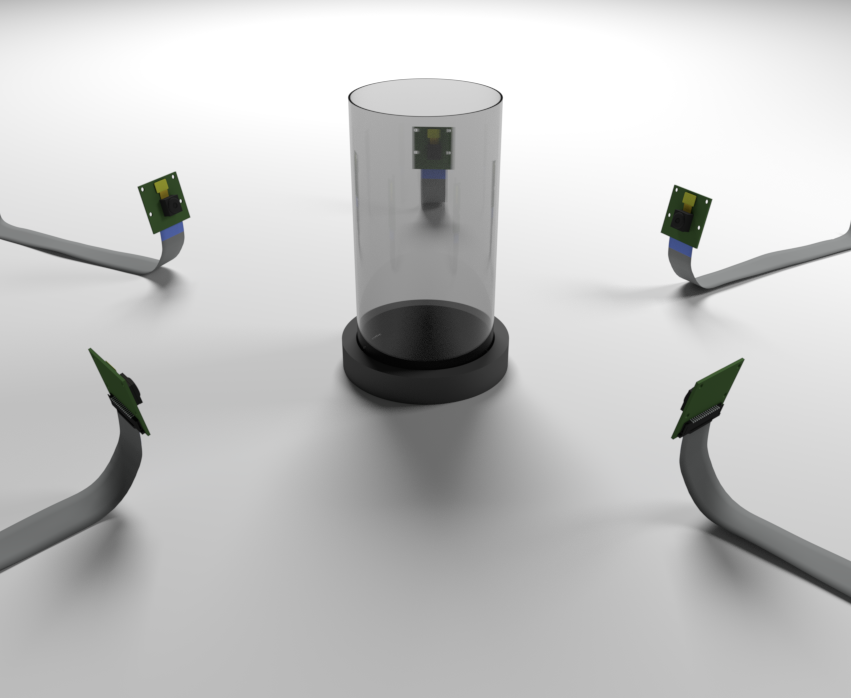
\includegraphics[width=0.95\textwidth]{images/renderCylinder.png}
		\caption{bisheriger Ansatz}
		\label{fig:oldSetup}
	\end{subfigure}%
	\begin{subfigure}{.5\textwidth}
		\centering
		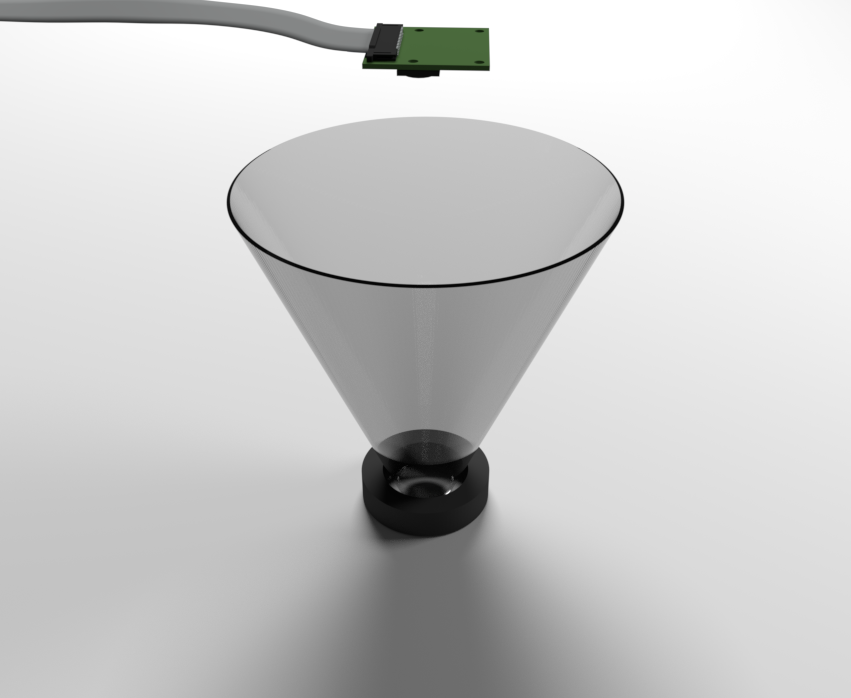
\includegraphics[width=0.95\textwidth]{images/renderCone.png}
		\caption{neuer Ansatz}
		\label{fig:newSetup}
	\end{subfigure}
	\caption{beide Ansätze im Vergleich}
	\label{fig:renderedSetup}
\end{figure}